\documentclass[conference]{IEEEtran}
% IEEE format with two-column layout

\usepackage[utf8]{inputenc}
\usepackage{amsmath,amssymb,amsthm,amsfonts}
\usepackage{graphicx}
\usepackage{subcaption}
\usepackage{url}
\usepackage{tikz}

\usepackage{booktabs}
\usepackage{url}
\usepackage{hyperref}
\usepackage{caption}

\usepackage{cite}

\usepackage{ulem}

\usepackage{algorithm}
\usepackage{algpseudocode}

\usepackage{mathtools}
\usepackage{etoolbox}

\makeatletter
\let\lunderbrace\underbrace
\let\runderbrace\underbrace
\let\lupbracefill\upbracefill
\let\rupbracefill\upbracefill
\patchcmd{\lunderbrace}{\upbracefill}{\lupbracefill}{}{}
\patchcmd{\runderbrace}{\upbracefill}{\rupbracefill}{}{}
\patchcmd{\lupbracefill}{\braceru}{\leaders\vrule\@height\ht\z@\@depth\z@\hskip\wd\z@}{}{}
\patchcmd{\rupbracefill}{\bracelu}{\leaders\vrule\@height\ht\z@\@depth\z@\hskip\wd\z@}{}{}
\makeatother

\usepackage{tikz}

\usepackage[a4paper,margin=1in]{geometry}

\usetikzlibrary{matrix,fit,positioning}

\title{\fontsize{18}{22}\selectfont Cool, Chill, and Cruel: Probabilistic Ranking with Greedy \\ Approach for Recovering Sparse Binary Secrets in LWE}
\author{\IEEEauthorblockN{MAMANCHUK Mykola, SID.202420671 \\ Supervising Professor: KUNIHIRO Noboru }
\IEEEauthorblockA{University of Tsukuba / CRISEC}
}
\date{\today}


\usetikzlibrary{matrix,fit,positioning}

% For good measure, define a geometry or margins if you prefer

\begin{document}
\maketitle

\begin{abstract}
    Sparse binary LWE secrets are widely used in homomorphic encryption (HE) and post-quantum cryptography due to their efficiency. However, recent attacks (e.g., SALSA, PICANTE, VERDE) show that ML and statistical methods can break such secrets at moderate dimensions. Classical lattice-based attacks reveal that after partial reduction, some LWE matrix columns remain high-variance ("cruel"), while others become low-variance ("cool").
    
    We introduce a three-zone approach—\textbf{Cruel, Chill, and Cool}—that refines this model. By combining brute force for cruel columns, ML-based probabilistic enumeration for chill columns, and greedy bit-flips for cool columns, we achieve a more flexible attack strategy. We analyze complexity, present schematic diagrams, and explore potential implications for RLWE, demonstrating that a three-region partition better exploits partially reduced matrices compared to prior two-region methods.
    \end{abstract}

    \section{Introduction}
    
    \subsection{Problem Statement and Existing Attacks}
    
    Cryptanalysis of sparse LWE secrets typically involves:
    \begin{itemize}
        \item \textbf{Primal and Dual attacks}: Dimensionality reduction and short-vector recovery \cite{primal-dual}.
        \item \textbf{Hybrid meet-in-the-middle (MiTM)}: Partial bit guessing combined with lattice reduction \cite{hybrid-mitm}.
        \item \textbf{ML-based attacks} (e.g., SALSA, PICANTE, VERDE): Identifying correct bits via neural networks and transformers \cite{salsa, picante, salsa-verde}.
    \end{itemize}
    
    These methods classify columns as either "hard" (high variance) or "easy" (low variance). However, in practice, variance decreases \emph{gradually}, forming a \textbf{sloping} region that doesn't fit into a strict two-zone model.
    
    \subsection{Our Contribution}
    
    We propose a refined three-zone approach—\textbf{Cruel, Chill, and Cool}—for sparse LWE key recovery:
    
    \begin{itemize}
        \item \textbf{Cruel region}: High-variance columns (\(\sim \frac{q}{12}\)), requiring brute force or meet-in-the-middle.
        \item \textbf{Chill region}: Moderate-variance columns handled via \emph{probabilistic or ML-based enumeration}, reducing brute-force overhead.
        \item \textbf{Cool region}: Low-variance columns, recoverable via greedy bit-flips.
    \end{itemize}
    
    This partitioning minimizes the search space in each zone. We provide complexity estimates, diagrams, and discuss RLWE implications, showing how this three-region method improves over traditional two-region attacks by leveraging ML-assisted partial recovery.    
  
  \section{Related Work}
  
  \subsection{Existing Lattice-Based Attacks}
  Several known attacks on small or sparse secrets include:
  \begin{itemize}
      \item Primal, Dual, and Hybrid attacks \cite{primal-dual, hybrid-mitm}.
      \item SALSA, a statistical attack leveraging machine learning \cite{salsa}.
      \item PICANTE, which incorporates transformer-based heuristics for LWE key recovery \cite{picante}.
      \item SALSA VERDE, an improved version of SALSA, refining its statistical recovery approach \cite{salsa-verde}.
  \end{itemize}
  
  \subsection{Inspiration for Our Work}
  This work was inspired by the recent research presented in \cite{cool-and-cruel}, which explored the effects of partial lattice reduction on LWE secrets and motivated the three-zone partitioning approach.
  
  \subsection{Conclusion}
  
  We introduce a novel three-zone attack strategy that extends existing binary LWE key recovery methods by partitioning reduced columns into **Cruel, Chill, and Cool** regions. This allows for an adaptive attack leveraging brute-force, probabilistic heuristics, and efficient greedy methods. Our analysis suggests that this approach can improve over traditional two-region models by better handling variance gradients in partially reduced lattices. Future work includes exploring its applicability to structured LWE variants such as Ring-LWE.
  
  \section{Preliminaries and Background}
  \label{sec:preliminaries}
  
  \subsection{Learning With Errors (LWE)}
  \label{subsec:lwe-def}
  
  LWE is defined by sampling:
  \begin{itemize}
      \item $\mathbf{A} \in \mathbb{Z}_q^{m \times n}$ (uniform),
      \item $\mathbf{s} \in D_s \subseteq \mathbb{Z}_q^n$ (secret),
      \item $\mathbf{e} \in D_e \subseteq \mathbb{Z}_q^m$ (small noise).
  \end{itemize}
  The challenge is to recover $\mathbf{s}$ from:
  \[
      \mathbf{b} \equiv \mathbf{A}\mathbf{s} + \mathbf{e} \pmod{q}.
  \]
  For **sparse binary LWE**, $\mathbf{s} \in \{0,1\}^n$ has Hamming weight $h$.
  
  \paragraph{Variants.} 
  Modifying $D_s, D_e$ leads to binary, ternary, Gaussian, or ring-based (RLWE) variants.
  
  \subsection{Partial Lattice Reduction}
  \label{subsec:partial-reduction}
  
  LWE is often attacked via \emph{partial lattice reduction} using the $q$-ary embedding:
  \[
  \Lambda =
  \begin{pmatrix}
  0 & qI_n \\
  \omega I_m & \mathbf{A}
  \end{pmatrix},
  \]
  where $\omega$ balances reduction strength vs. noise amplification. Applying BKZ, \texttt{flatter}, or \texttt{polish} yields:
  \[
  \mathbf{A}' = \mathbf{R}\mathbf{A}, \quad \mathbf{b}' = \mathbf{R}\mathbf{b}.
  \]
  Reduction quality is measured by:
  \[
    \rho = \frac{\sigma(\mathbf{A}')}{\sigma(\mathbf{A}_{\text{init}})}, 
    \quad \sigma(\mathbf{A}_{\text{init}}) = \frac{q}{\sqrt{12}}.
  \]
  Lower $\rho$ indicates better reduction but may increase noise.
  
  \begin{figure}[ht]
    \centering
    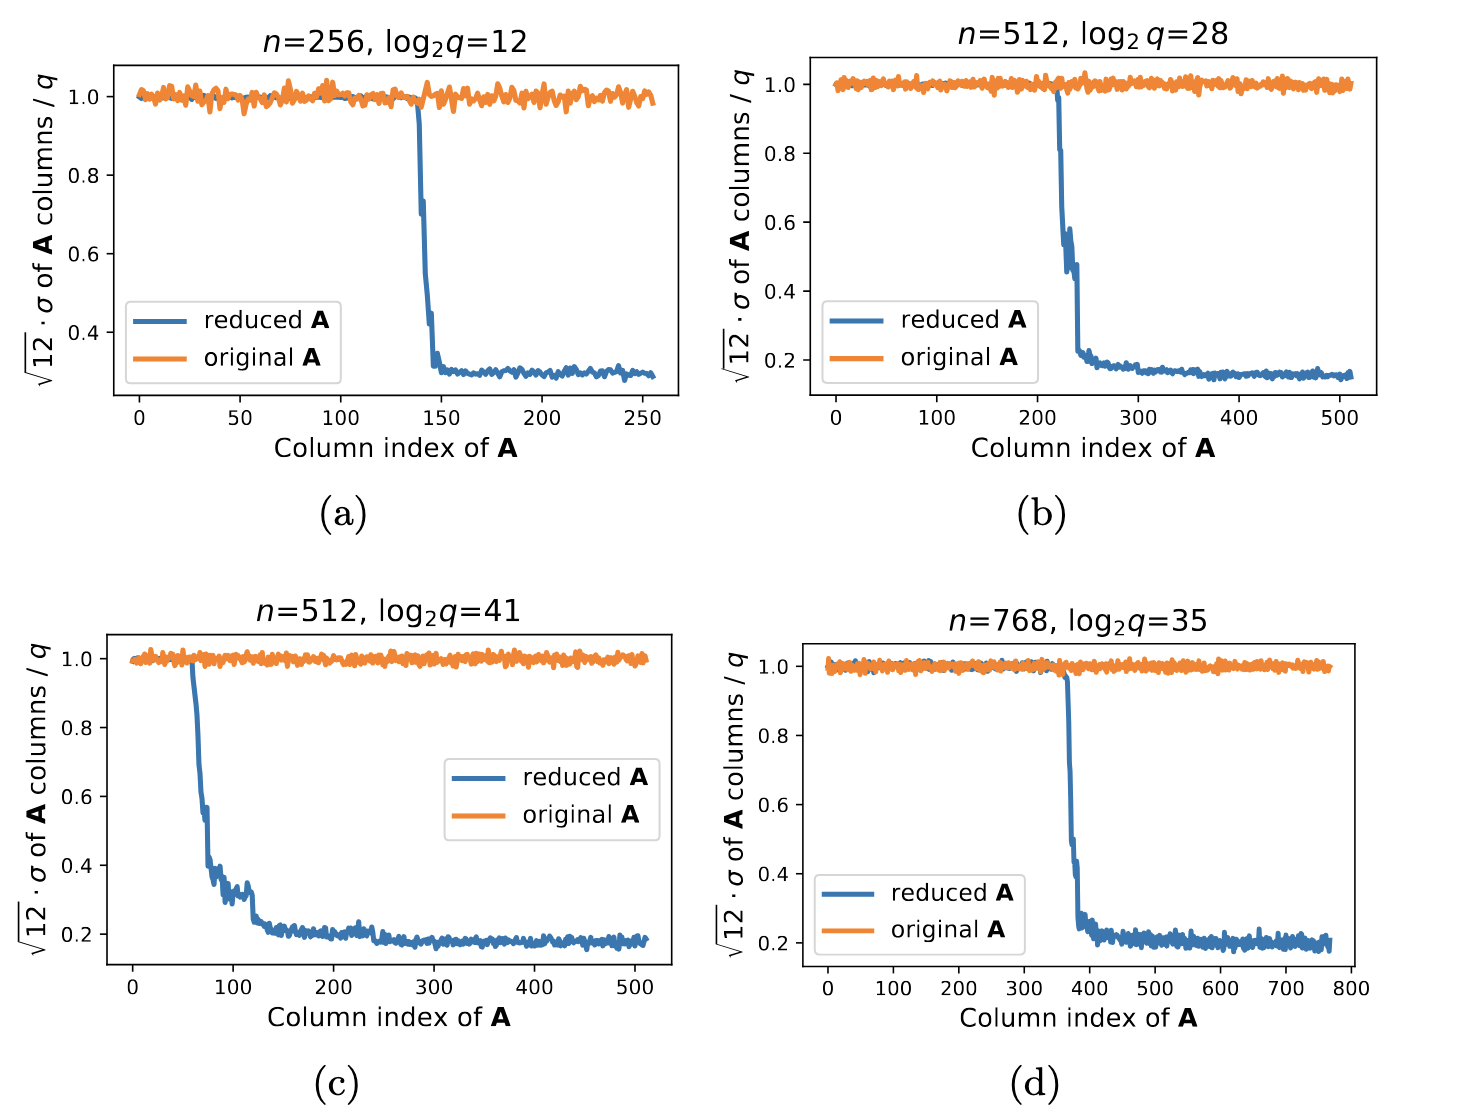
\includegraphics[width=1\linewidth]{example_variance_plot.png} 
    \caption{\small Variance separation: original $\mathbf{A}$ (orange) vs. reduced $\mathbf{A}$' (blue), with a drop at index $n_u$.}
    \label{fig:variance-separation}
  \end{figure}
  
  \paragraph{Sub-Sampling \& Interleaving.}
  Often, $m$ is sub-sampled from $4n$+ LWE samples. Reduction techniques like BKZ and \texttt{flatter} may be interleaved, with termination based on $\rho$ convergence.
  
  \subsection{Greedy Recovery of ``Cool'' Bits}
  \label{subsec:greedy}
  
  Following \cite{cool-and-cruel}, after solving the high-variance ("cruel") subset, the remaining low-variance ("cool") columns can be recovered efficiently using \emph{greedy bit-flips}. We summarize this as **Algorithm~1**.
  

\begin{algorithm}[ht]
\caption{\small Greedy Recovery of Cool Bits (from \cite{cool-and-cruel})}
\label{alg:greedy-cool}
\begin{algorithmic}[1]
\Require $\mathbf{s}^*$ partially known (correct cruel bits); the rest initially $=0$.
\For{$i \in \{n - n_r, \ldots, n-1\}$}
  \State $s^*[i] \gets 0$
  \State $\sigma_0 \gets \sigma(\mathbf{A}\cdot \mathbf{s}^* - \mathbf{b}\mod q)$
  \State $s^*[i] \gets 1$
  \State $\sigma_1 \gets \sigma(\mathbf{A}\cdot \mathbf{s}^* - \mathbf{b}\mod q)$
  \If{$\sigma_0 \le \sigma_1$}
    \State $s^*[i] \gets 0$
  \Else
    \State $s^*[i] \gets 1$
  \EndIf
\EndFor
\end{algorithmic}
\end{algorithm}

\noindent
\textbf{Interpretation.}
We individually check whether flipping a particular bit from $0$ to $1$ lowers the residual’s variance; if so, we keep that flip.
This linear-time method works well when each column has \emph{significantly reduced} variance, ensuring a strong statistical signal per bit.

\begin{figure}[ht]
  \centering
  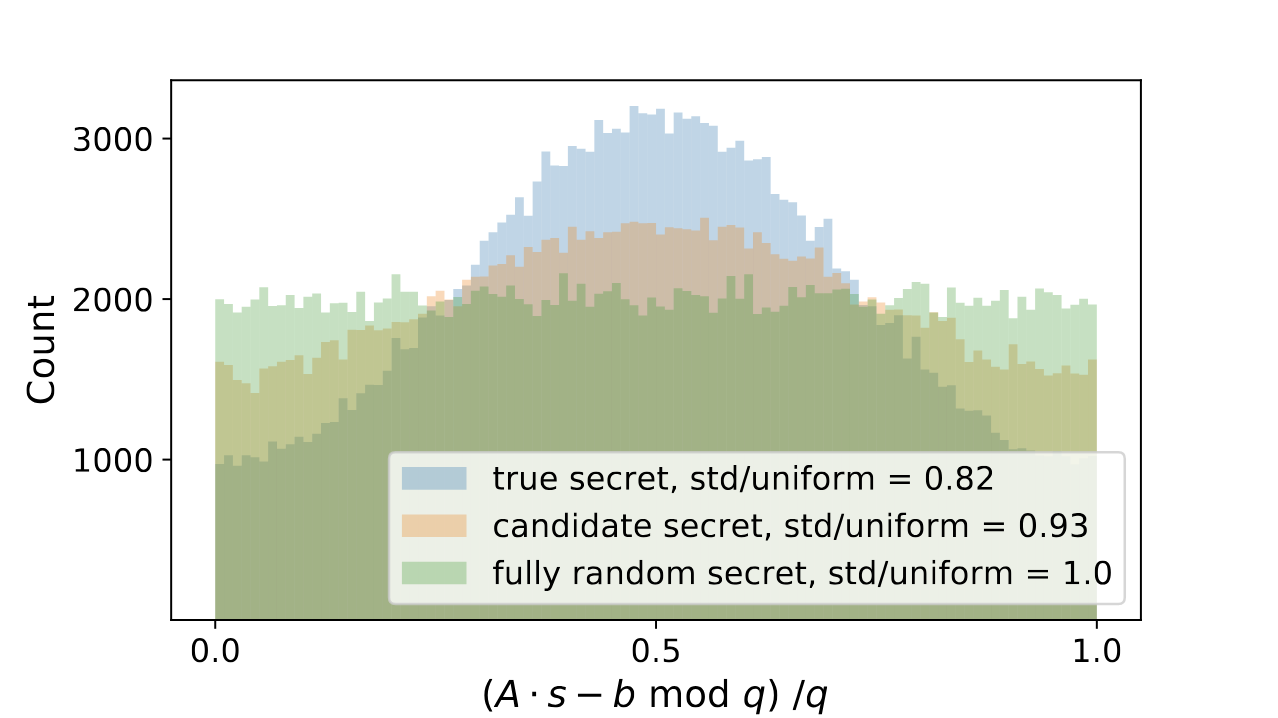
\includegraphics[width=1\linewidth]{residual_histogram.png}
  \caption{\small Residual histograms mod $q$.  
    \textbf{Blue:} True secret guess (narrow distribution),  
    \textbf{Orange:} Partially correct guess (e.g., cruel bits only),  
    \textbf{Green:} Random guess (near-uniform).}
  \label{fig:residual-histograms}
\end{figure}

\paragraph{Limitations.}
When a subset of columns has only \emph{moderately} reduced variance (``sloping''), flipping bits individually can fail if noise remains too large. 
Hence, our proposal in Section~\ref{sec:proposed-ccc} extends beyond a pure \emph{cruel/cool} partition, introducing a ``chill'' region for partial or probabilistic enumeration.

een purely h\section{Variance Diagram and Motivation for a Three-Zone Partition}
\label{sec:3zone-motivation}

\subsection{Empirical Observation}
After applying partial lattice reduction to the LWE matrix $\mathbf{A}$, the column-by-column standard deviation often exhibits a near-vertical ``cliff''. However, we observe that in some cases, the transition between high variance and low variance can form a \emph{sloping} region, shown in Figure~\ref{fig:variance-annotated}.

\begin{figure}[ht]
    \centering
    \begin{subfigure}{0.49\textwidth}
        \centering
        % Insert your actual figure path:
        \begin{tikzpicture}
            \node[anchor=south west, inner sep=0] (image) at (0,0)
              {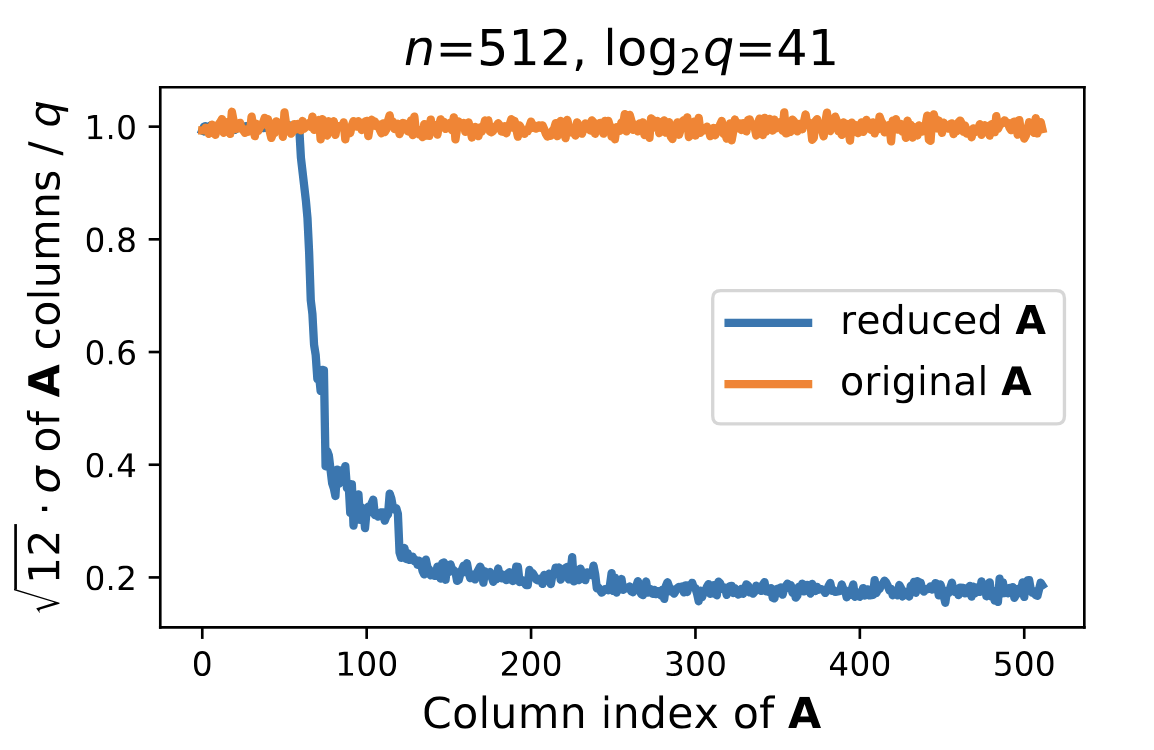
\includegraphics[width=\textwidth]{512-41.png}};
            \begin{scope}[x={(image.south east)}, y={(image.north west)}]
                % Cruel region (green frame)
                \draw[thick, green, fill=green!20, opacity=0.3] (0.18, 0.19) rectangle (0.28, 0.8);
                % Chill region (yellow frame)
                \draw[thick, yellow, fill=yellow!20, opacity=0.3] (0.285, 0.19) rectangle (0.345, 0.8);
                % Cool region (blue frame)
                \draw[thick, blue, fill=blue!20, opacity=0.3] (0.35, 0.19) rectangle (0.91, 0.8);
            \end{scope}
        \end{tikzpicture}
        \caption{\small $n=512, \log_2 q=41$.}
        \label{fig:region1}
    \end{subfigure}
    \hfill
    \begin{subfigure}{0.49\textwidth}
        \centering
        % Insert your actual figure path:
        \begin{tikzpicture}
            \node[anchor=south west, inner sep=0] (image) at (0,0)
              {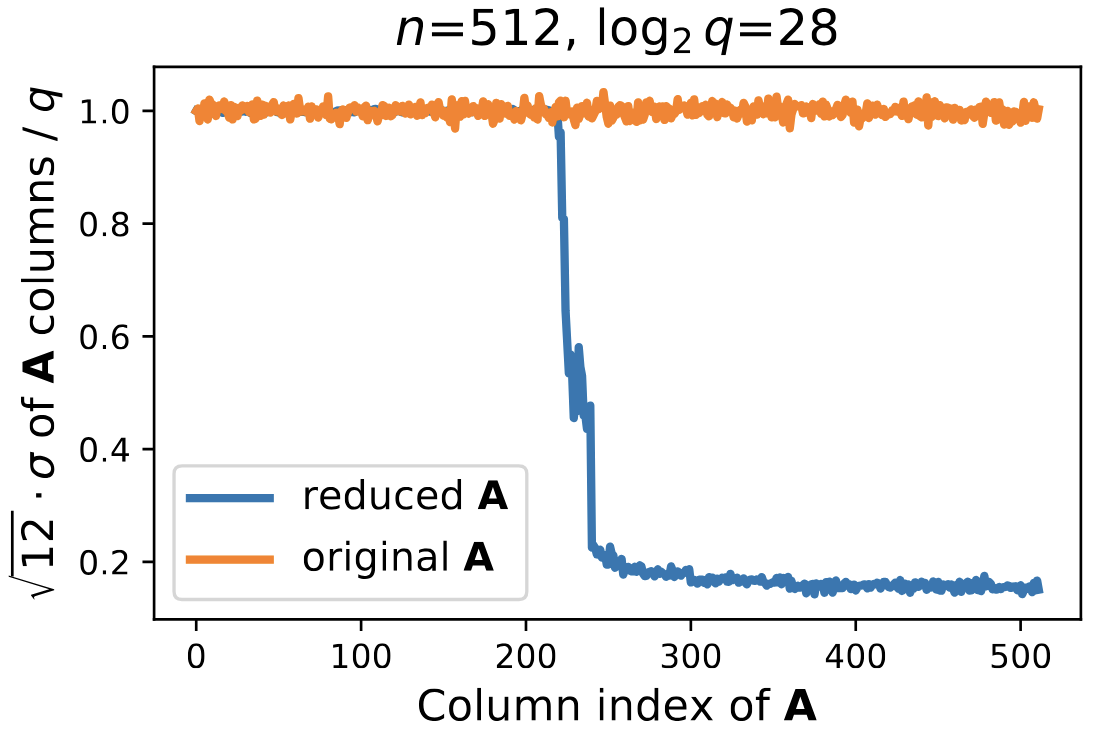
\includegraphics[width=\textwidth]{512-28.png}};
            \begin{scope}[x={(image.south east)}, y={(image.north west)}]
                % Cruel region (green frame)
                \draw[thick, green, fill=green!20, opacity=0.3] (0.18, 0.19) rectangle (0.505, 0.8);
                % Chill region (yellow frame)
                \draw[thick, yellow, fill=yellow!20, opacity=0.3] (0.510, 0.19) rectangle (0.525, 0.8);
                % Cool region (blue frame)
                \draw[thick, blue, fill=blue!20, opacity=0.3] (0.530, 0.19) rectangle (0.935, 0.8);
            \end{scope}
        \end{tikzpicture}
        \caption{\small $n=512, \log_2 q=28$.}
        \label{fig:region2}
    \end{subfigure}
    \caption{\small Empirical plots of column standard deviation (scaled by $\sqrt{12}/q$) before and after reduction, annotated with \textbf{Cruel} (green), \textbf{Chill} (yellow), and \textbf{Cool} (blue) regions. 
    In some instances (left subfigure), the transition from high variance to low variance is relatively narrow, while in others (right subfigure), it forms a longer slope.}
    \label{fig:variance-annotated}
\end{figure}
\paragraph{Why a Slope Can Appear.}
Depending on how \texttt{flatter}, BKZ, or other reduction algorithms interleave, the final column norms might not transition abruptly from $\approx q/\sqrt{12}$ to a fully reduced state. Instead, a fraction of columns may exhibit intermediate ``semi-reduced'' variance, producing what we refer to as a \emph{sloping region}.

\subsection{Why a Three-Zone Partition?}
\label{subsec:3zone}

Historically, ``Cool \& Cruel'' style attacks assumed columns are either:
\begin{itemize}
    \item \emph{Cruel:} High variance $\approx q/\sqrt{12}$, needing brute force or meet-in-the-middle;
    \item \emph{Cool:} Low variance, quickly recovered via bit-flip or minimal overhead.
\end{itemize}
However, a purely two-zone approach \emph{misses} the subtle \emph{middle} region where variance is neither clearly high nor fully reduced. We propose a three-zone decomposition:
\vspace{-5mm}
\[
  \mathcal{I}_{\mathrm{cruel}},\;
  \mathcal{I}_{\mathrm{chill}},\;
  \mathcal{I}_{\mathrm{cool}}
  \;\subseteq\;\{1,\ldots,n\}, 
  \;\;
\]
\vspace{-8mm}
\[
  \mathcal{I}_{\mathrm{cruel}}\cup\mathcal{I}_{\mathrm{chill}}\cup\mathcal{I}_{\mathrm{cool}}=\{1,\ldots,n\}.
\]

\begin{itemize}
    \item \textbf{Cruel (green)}:  
    High-variance columns (\(\mathbf{A}_{*,j} \sim q/\sqrt{12}\)), requiring brute force or hybrid guessing. 
    \item \textbf{Chill (yellow)}:  
    Transitional columns with moderate variance, handled via probabilistic or ML-based methods.  
    \item \textbf{Cool (blue)}:  
    Low-variance columns, recoverable via greedy bit flips.
\end{itemize}
  

Next section formalizes the details of each zone’s attack strategy.

\section{Proposed Method: \texorpdfstring{Cool, Chill, and Cruel}{Cool, Chill, and Cruel}}
\label{sec:proposed-ccc}

\subsection{Threshold-Based Zoning}
\label{subsec:threshold-zoning}

After partially reducing the LWE matrix $\mathbf{A}'$ (Section~\ref{subsec:partial-reduction}), each column $j$ has an associated standard deviation $\sigma_j$. We define two thresholds $T_c$ and $T_h$ with 
\[
  T_c > T_h > 0,
\]
for instance $T_c \approx 0.8 \,\sigma_u$ and $T_h \approx 0.3\, \sigma_u$, where $\sigma_u \approx \frac{q}{\sqrt{12}}$ is the original uniform standard deviation. Then, each column $j$ is classified into one of three regions:
\[
  \mathrm{Region}(j) \;=\;
  \begin{cases}
    \text{Cruel}, & \text{if } \sigma_j \;\ge\; T_c,\\
    \text{Chill}, & \text{if } T_h \;\le\; \sigma_j < T_c,\\
    \text{Cool}, & \text{if } \sigma_j \;<\; T_h.
  \end{cases}
\]
This yields three disjoint subsets $\mathcal{I}_{\mathrm{cruel}}, \mathcal{I}_{\mathrm{chill}}, \mathcal{I}_{\mathrm{cool}} \subseteq \{1,\ldots,n\}$.

\subsection{Attack Phases}
\label{subsec:attack-phases}

Our attack proceeds in three phases based on column variance:

\begin{itemize}
  \item \textbf{Phase 1: Brute Force (Cruel)} – High-variance columns \(\mathcal{I}_{\mathrm{cruel}}\) are guessed via brute-force or meet-in-the-middle:
    \[
    \mathbf{s}_{\mathrm{cruel}} = \mathrm{BruteForceCruel}(\mathbf{A}_{*, \mathcal{I}_{\mathrm{cruel}}}, \mathbf{b})
    \]
    with \(\mathrm{cruel\_ones} = \mathrm{HW}(\mathbf{s}_{\mathrm{cruel}})\) denoting the recovered 1-bits.

  \item \textbf{Phase 2: Probabilistic Enumeration (Chill)} – Medium-variance columns \(\mathcal{I}_{\mathrm{chill}}\) are ranked by probability:
    \[
    p_j = \mathrm{EstimateProb}(j, \mathbf{A}, \mathbf{s}_{\mathrm{cruel}})
    \]
    and \( k = h - \mathrm{cruel\_ones} \) bits are assigned via ranking, with local flips used if refinement is needed.

  \item \textbf{Phase 3: Greedy Bit-Flip (Cool)} – Low-variance columns \(\mathcal{I}_{\mathrm{cool}}\) are solved with \textproc{GreedyFlip}, flipping bits to minimize residual deviation.
\end{itemize}

\subsection{Pseudocode: Multi-Zone Recovery}
\label{subsec:multi-zone-pseudocode}

\begin{algorithm}[ht]
\caption{\small Multi-Zone Attack: Cool, Chill, and Cruel}
\label{alg:ccc-attack}
\begin{algorithmic}[1]
\Require Reduced matrix $\mathbf{A}$, vector $\mathbf{b}$, modulus $q$, Hamming weight $h$
\State $(\mathcal{I}_{\mathrm{cruel}},\;\mathcal{I}_{\mathrm{chill}},\;\mathcal{I}_{\mathrm{cool}}) \;\gets\; \text{ClassifyColumns}(\mathbf{A}, T_c, T_h)$
\State $\mathbf{s}_{\mathrm{cruel}} \gets \mathrm{BruteForceCruel}(\mathbf{A}_{*,\mathcal{I}_{\mathrm{cruel}}}, \mathbf{b})$
\State $\mathrm{cruel\_ones} \gets \mathrm{HW}(\mathbf{s}_{\mathrm{cruel}})$
\State $p_j \gets \mathrm{EstimateProb}(j,\mathbf{A},\mathbf{s}_{\mathrm{cruel}})\; \forall j\in \mathcal{I}_{\mathrm{chill}}$
\State $k = h - \mathrm{cruel\_ones}$, $\mathbf{s}_{\mathrm{chill}} \gets \mathrm{RankAndAssign}(p_j,k)$
\State $\mathbf{s}_{\mathrm{cool}} \gets \mathrm{GreedyFlip}(\mathbf{A},\mathbf{b},\mathbf{s}_{\mathrm{cruel}},\mathbf{s}_{\mathrm{chill}})$
\State $\mathrm{RefineChill}(\mathbf{A},\mathbf{b},\mathbf{s}_{\mathrm{cruel}},\mathbf{s}_{\mathrm{chill}},\mathbf{s}_{\mathrm{cool}})$
\State \textbf{return} $(\mathbf{s}_{\mathrm{cruel}},\;\mathbf{s}_{\mathrm{chill}},\;\mathbf{s}_{\mathrm{cool}})$
\end{algorithmic}
\end{algorithm}

\paragraph{Implementation Notes.}
\begin{itemize}
\item \textproc{EstimateProb} ranks chill columns using variance or ML-based probability estimation.
\item \textproc{RankAndAssign} selects the top \( k \) chill bits as 1, refining with flips if needed.
\item \textproc{GreedyFlip} minimizes residual deviation by adjusting low-variance bits.
\end{itemize}

Each region is handled according to its variance, balancing brute force, ML ranking, and greedy recovery to optimize efficiency and success probability.

\section{Mathematical and Logical Details}
\label{sec:math-logic}

\subsection{Probability and Complexity Insights}
\label{subsec:prob-comb}

Given a classification into \emph{Cruel, Chill,} and \emph{Cool} regions with respective counts $n_{\mathrm{cruel}}, n_{\mathrm{chill}}, n_{\mathrm{cool}}$, we define:
\[
  \mathrm{cruel\_1} = \mathrm{HW}(\mathbf{s}_{\mathrm{cruel}}), \quad 
  k = h - \mathrm{cruel\_1}.
\]
where $h$ is the total Hamming weight. The remaining $k$ bits must be assigned within $\mathcal{I}_{\mathrm{chill}}$ and $\mathcal{I}_{\mathrm{cool}}$.

To determine which $\mathcal{I}_{\mathrm{chill}}$ columns contain 1s, each column $j \in \mathcal{I}_{\mathrm{chill}}$ is ranked by:
\[
  p_j = \Pr[s_j = 1],
\]
where $p_j$ can be estimated heuristically ($p_j \propto 1/\sigma_j$), via a small ML model (logistic regression or neural net on residuals), or through direct statistical tests. The top $k_{\mathrm{chill}} \leq k$ ranked columns are set to 1, with the remainder placed in the cool set.

If the initial classification is incorrect, a local search (BFS or iterative bit-flip) refines borderline assignments without fully enumerating $\binom{n_{\mathrm{chill}}}{k_{\mathrm{chill}}}$. 

\paragraph{Complexity Estimation.}  
The attack cost combines:
\[
  2^{n_{\mathrm{cruel}}} + \binom{n_{\mathrm{chill}}}{k_{\mathrm{chill}}} \times \text{ML\_overhead} + O(n_{\mathrm{cool}}),
\]
where the brute force term dominates for large $n_{\mathrm{cruel}}$, while the chill region overhead depends on partial enumeration and ranking efficiency.

\vspace{1em}
\noindent\textbf{Notional Complexity Formula.}
\begin{align*}
\mathbf{C}(n, k)
  &\approx\; 
  2^{n_{\mathrm{cruel}}} 
  \;+\;
  \binom{\textstyle n_{\mathrm{chill}}}{\textstyle k_{\mathrm{chill}}}
  \times\; \mathrm{ML\_overhead}(1) 
  \times\;
\end{align*}

\vspace{-5mm}

\noindent
\begin{align*}
    &\times\;
    \Bigl[
    1 \;+\; \mathrm{liability\_coef}
        \;\times\;
        \bigl(
          n \;-\; n_{\mathrm{cruel}} \;-\; n_{\mathrm{chill}}
        \bigr)
  \Bigr].
\end{align*}

\paragraph{Term-by-Term Explanation}
\begin{enumerate}
  \item \( 2^{n_{\mathrm{cruel}}} \):  
    Exhaustive or meet-in-the-middle enumeration for high-variance columns.

  \item \( \binom{n_{\mathrm{chill}}}{k_{\mathrm{chill}}} \):  
    Enumerations for selecting 1-bits in the chill region, mitigated by ranking or BFS.

  \item \( \mathrm{ML\_overhead}(1) \):  
    Overhead per candidate guess, from ML or statistical checks.

  \item \( \mathrm{liability\_coef} \times (\dots) \):  
    Models local flips or re-runs in the chill region.

  \item \textbf{Cool overhead}:  
    Typically \( O(n_{\mathrm{cool}}) \), from bit-flip verification in a reduced domain.
\end{enumerate}

\paragraph{Comparison to Original Cool-and-Cruel}
In \cite{cool-and-cruel}, columns are labeled as \textbf{hard} (\( n_u \) brute-force bits) or \textbf{easy} (linear-time flips), with complexity:
\[
  2^{n_{u}} + O(n - n_u),
\]
where \( n_u \approx n_{\mathrm{cruel}} \).

This method struggles with \textit{medium-variance columns}, while our \textbf{three-zone} approach lowers \( n_{\mathrm{cruel}} \) via partial enumeration (\( \binom{n_{\mathrm{chill}}}{k_{\mathrm{chill}}} \)) or ML, reducing brute-force cost at the expense of chill-region overhead.

\section{Discussion, Future Work, and Conclusion}
\label{sec:discussion-future-conclusion}

\subsection{Discussion}
Our three-zone (\emph{Cruel}, \emph{Chill}, \emph{Cool}) approach refines partial lattice reduction by isolating a \emph{Chill} region to handle medium-variance columns. We aim to reduce search space while maintaining efficiency. Section~\ref{sec:math-logic} showed how Chill enumerations replace excessive brute force at some overhead cost.

\paragraph{Balancing Lattice Reduction.}
Stronger reduction lowers $n_{\mathrm{cruel}}$ but amplifies noise $\sigma_e$, affecting Chill/Cool classification \cite{cool-and-cruel}. An adaptive approach—tuning penalty parameter $\omega$ and BKZ/\texttt{flatter} block sizes—may balance enumeration complexity and error impact.

\subsection{Future Work}
\paragraph{1.\ Ternary/Gaussian Secrets.}
Extending Chill classification to ternary or Gaussian secrets requires adjusting probability estimates or separate ML models. Partial reduction depth may complicate recovery for multi-valued secrets.

\paragraph{2.\ Integrating SALSA or Transformers.}
ML-based methods (e.g., SALSA, PICANTE, VERDE) could improve Chill classification. However, managing ML overhead is critical to prevent excessive complexity increases.

\paragraph{3.\ Real-World HE Libraries.}
Homomorphic encryption libraries (HElib, SEAL) use small or sparse secrets. Mitigations, such as randomized secret distributions or enforced minimum Hamming weights, should be analyzed to assess real-world impact.

\paragraph{4.\ Parameter Tuning and Local Search.}
Optimizing local flips and BFS expansions in Chill is an open problem. Formalizing cost functions and iteration bounds could further reduce complexity.

\paragraph{5.\ Incremental Chill Expansion.}
Dynamically adjusting Chill vs. Cool classification based on success rates may improve efficiency. Experimental validation is needed to optimize runtime and accuracy.

\begingroup
Implementation will build on the original Cool and Cruel framework \cite{lwe-benchmarking}.
\endgroup

\subsection{Conclusion}
We introduced a \emph{Cruel, Chill, Cool} partition to refine LWE key recovery, balancing brute force, ML-based ranking, and bit-flipping. While Chill adds complexity, it reduces the need for excessive brute-force searches. 

Future work includes tuning lattice reduction depth ($\omega$), improving ML classification for Chill columns, and refining local search. Empirical tests up to $n=1024$+ will evaluate feasibility against real-world encryption libraries. Combining cryptanalytic strategies with ML insights may enhance attacks on small or sparse LWE secrets.

  \bibliographystyle{plain}
  \bibliography{references}

\end{document}